\chapter[Count time series aberration techniques]{Count time series analysis of the GTD}
\chaptermark{Outbreak detection}

\section{Introduction}
\label{sec:chap5intro}

A preliminary understanding of the GTD was gained through examining the data through the use of descriptive statistical visualization (using time series plots, geo-spatial plots, stacked bar plots), dimensional reduction techniques and unsupervised learning techniques and supervised techniques. An insight was gained into the underlying trends around temporal, spatial temporal, attack, weapon type and regio-specific significance (rural/urban divide) of terrorism. 

From the various descriptive visualizations it could be seen that post 2000, the Middle East and North Africa (particularly Iraq and Syria), along with South Asia (particularly Afghanistan) as being the pre-eminent regions in terms of deaths due to terrorism. As these were the predominant areas and countries in terms of deaths due to terrorism, they were selected for further analysis using supervised and unsupervised methods. This information is held in Apendix~\ref{sec:appendixprelim}.

In the preliminary modelling work the number of deaths due to terrorism in Iraq was modelled using count regression to examine the underlying correlation or relationships between a number of explanatory variables. These were 
\begin{itemize}
\item Major US and NATO strategic actions, i.e. invasion of Iraq, the troop surge in 2007, the pull out, the launch of inherent resolve to combat ISIS etc.
\item Iraqi presidential reign.
\item Month Post 1970.
\end{itemize}

However the count modelling suffered from the models not being correctly specified, with count specific modelling techniques suffering from over dispersion. While linear and robust regression techniques applied to the count data required the data to be log transformed and again the models appeared to be specified incorrectly.   

The number of counts (of deaths due to terrorism in Iraq) were also modelled using HMM's which proved to be very useful in terms of time series analysis by being able to ascertain different epochs (regions in time time of high probability of high or low terrorism counts of deaths due to terrorism) of counts of deaths of terrorism. Through the use of a simple transformation these transition state probabilities can be transformed into classes of non-terror or terror epochs, making the HMM easier to interpret (see figure~\ref{fig:Rplot02_2008_facstate_HMM}). Such a model would be useful for modelling outbreaks of terrorism and would have applications in a number of areas from risk management to enabling counter terrorism/counter insurgency policies. However the models as they were unsupervised required the number of states to be decided before hand or be empirically derived. Therefore the use of these algorithms for detecting  on a country by country (or even the preference of a particular analyst for a particular country) basis would be difficult.

\section{Outbreaks, syndromes and anomalies in  time series count data} 

Anomaly detection, outbreak detection and medical surveillance methods can act as an intelligent filter to highlight ‘interesting events’ in terms of count time series data. These filters are necessary to prevent overloading an analyst with information and serve to place in the spotlight the observations that are the most different (and least like) the main population and focus attention on the most surprising or unanticipated results. These anomalies can be interesting or unexpected in two ways, they can be vertically or horizontally uncharacteristic. Vertically uncharacteristic observations would be sudden spikes, while a horizontally uncharacteristic observation would be a stepwise change (a typical stepwise change would be a mean shift) or a ramp up.

A breakout is defined by 2 steady states and an intermediate transition period. Breakout detection is usually accomplished using two means. These are:
\begin{itemize}
\item Mean shift. This is where an abrupt change in what is being assessed by the modelling technique (in the context of this research this would either be deaths due to terrorism or terrorist incidents) is detected. 
\item Ramp up. This is where a slow and steady increase in the variable being studied from one state to another occurs.
\end{itemize}

Breakout detection algorithms have a wide use and have been applied to everything from monitoring disease outbreaks to emerging trends on social media.

Medical syndromic surveillance methods (such as the Farrington or EARSC algorithm used in this research) are used in syndromic medical surveillance. A syndrome can be defined as a collection of symptoms or conditions that happen concurrently and correlate highly with the presence of a disease or a higher probability of catching a disease. Syndromic surveillance is aimed at detecting changes in time series counts of certain symptoms for the early warning and detection of a possible outbreak of disease. These algorithms are designed to provide an alarm of a possible outbreak not to confirm that an outbreak has occurred or why it has.

Time series outlier detection can be used to detect time series events which appear different from the the overall trend, these may manifest themselves as (positive) sudden spikes or troughs in count data.

The benefits to using these methodologies in the detection of changes in intensity of terrorist activity is that they are highly generalizable as the numbers of tunable parameters are small and the resulting outbreaks, outliers and syndromic outbreaks can be correlated to real world events. Another benefit of using these methods is that they act as a compliment of each other
identifying different time-count events. For instance an outlier may be detected in the absence of an outbreak (or syndromic surveillance outbreak) which would indicate it to be an aberration not a step change or a time event which may indicate a more serious sustained outbreak.

Providing this data to an analyst allows him to marry objective criteria with his own expert (and subjective) knowledge as to whether an aberration has occurred or if something far more serious is taking place, for example a break out in terrorism which is symptomatic of major insurgent activity. In this way, using the algorithms in conjunction with each other they can act as an intelligent filter to an analyst only highlighting the \textit{'most interesting'} events. 

Finally syndromic surveillance and outbreak detection can detect the effect of a particular intervention and if it has a positive effect ( in the context of this research this would translate to a mean or gradual shift down in terrorist deaths, or a drop off in outbreaks) in this  way it provides an analyst with greater situational awareness about the effectiveness of particular interventions. 

\section{Algorithms used for modelling time series count data and their methodology}

Four models were initially trialled, two were anomaly detection algorithms (twitter outbreak detection algorithm SURUS and RAD) and two were outbreak detection algorithms used in disease outbreak monitoring, the EARSC and Farrington algorithm and are classed as medical surveillance algorithms. 

\subsection{Online time series outbreak and anomaly detection algorithm}
The underlying algorithm utilized by the twitter outbreak detection algorithm \citep{twitterooutbreak} is E-Divisive with Medians \citep{james2014leveraging}  which makes use of energy statistics to figure out when a large departure from the median has occurred. EDM has a number of advantages for outbreak detection, such as, it is robust when anomalies are present in the data. EDM has the following characteristics:
\begin{enumerate}
\item EDM as stated above utilizes robust statistical measures, the median and approximates the statistical importance of a breakout through availing of a permutation test.
\item EDM is non-parametric, the underlying distribution of count data does not have to be known.
\end{enumerate}

The twitter outbreak detection algorithm makes use of a weighted $L^{2} distance$. The $L^{2} distance$  of X and Y (which are independent random variables) and X' and Y' which are their relevant i.i.d copies, is given by equation~\ref{eq:energystatistic1}.

\begin{equation} \varepsilon (X,Y) = 2E|X-Y|-E|X-X'|-|Y-Y'| \label{eq:energystatistic1}  \end{equation} 

The $L^{2} distance$  between the cumulative distribution functions of X and Y which are represented by F and G is given by equation~\ref{eq:energystatistic2}. 

\begin{equation} 
2\int_{-\infty}^{\infty} (F(x)-G(x))^2 dx = \varepsilon (X,Y)
\label{eq:energystatistic2}  \end{equation} 

For X, its characteristic function is described by equation~\ref{eq:energystatistic3}

\begin{equation} 
\phi_{x}(t)=E(exp(iXt))
\label{eq:energystatistic3}  \end{equation}

Based on equation~\ref{eq:energystatistic3} the energy distance can be written in terms of characteristic functions as equation~\ref{eq:energystatistic4} 

\begin{equation} 
\varepsilon (X,Y) =\int_{-\infty}^{\infty} \frac{|\phi_{x}(t)-\phi_{y}(t)|^2}{\pi t^2} dt.
\label{eq:energystatistic4}  \end{equation} 

Since the cumulative function similarly to the characteristic function (equation~\ref{eq:energystatistic4}) specifies a random variable, a class distance measure can be defined by equation~\label{eq:energystatistic5},

\begin{equation} 
D(X,Y;\alpha)=\int_{-\infty}^{\infty}|\phi_x(t)^2-\phi_y(t)|^2 \epsilon \omega(t:\alpha) dt
\label{eq:energystatistic5}  \end{equation} 

Where $\omega(t:\alpha)$ is a weight function described by the indexing parameter $\alpha$. $\alpha$ is utilized to account for the distance intermediate between the distributions, where $D(X,Y;\alpha)<\infty$

Time series outlier detection can be seen  as a complementary methodology to outbreak detection. To carry out outlier detect on our data Robust PCA (RPCA) is used \citep{zhou2010stable}. Matrix decomposition has been previously used in the exploratory analysis section, in chapter 4 matrix decomposition through the use of MCA was used to examine the associations between different categorical variables. Upon performing RPCA on a dataset, a decomposition is calculated of the form (equation~\ref{eq:robustRPCA}, where x is the decomposition, L is the low-rank matrix, S a sparse matrix and E is a dense error matrix)

\begin{equation} 
X =L+S+E
\label{eq:robustRPCA}  \end{equation} 

In this analysis, Netflix's RAD (Robust Anomaly Detection)  \citep{RAD2017} is used to identify the least related time series count events within a larger dataset. In the RAD algorithm an array of features is determined for each time series, which calculate different components of the series, including lag correlation (the correlation between the series and a series with a lag of a certain period derived from the same series), the amount of seasonality and spectral entropy ( which describes the complexity of a series). PCA is then preformed on the features followed by the application of a number of bivariate outlier detection methods based on highest density regions and $\alpha$ hulls applied to the first two principal components to identify outliers. Again, the benefit to using Netflix's RAD algorithm is its application can be generalized very easily, as very few parameters are required to tune the algorithm.
 
\subsection{Surveillance algorithms}

In the field of medical statistics univariate time series of count data are readily available methodologies for for surveying outbreak of medically related incidents, these form the basis of (medical) surveillance problems. Two of the most common surveillance methods Farrington's \citep{farrington1996statistical} and the EARSC algorithms \citep{fricker2008comparing} were applied to the problem of modelling count of deaths due to terrorism to test their suitability for determining outbreaks of terrorist activity (counts of deaths due to terrorism).

The two methodologies used in this analysis available in the surveillance package \citep{surveillancepackageR} were:

\begin{itemize}
\item Farrington's Method, the algorithm farrington or farringtonFlexible (surveillance package).
\item  EARSC Method (EARSC3), the algorithm EARSC3 (surveillance package).
\end{itemize}

\subsection{Farrington's Method}
Farrington's methodology \citep{salmon2016monitoring} is  used to predict the actual value of counts of incidents $y_{n}$ using a unique collection of reference values taken from the observed values $y_{1}..y_{n-1}$, to account for far reaching trends and seasonality, values are only selected from a window of size $2w+1$ at time n for b years in the past. This has the effect of only selecting a set of recent values with comparable properties at a time and can be stated as (equation~\ref{eq:farringtoneq1})
where r is the period from which the observations were taken from. Poisson regression accounting for over dispersion is then used to model the $(2w+1)B$, reference sample, \citep{robertson2010review}.


\begin{equation} 
R(w,b)=(\bigcup_{i=1}^{b}\bigcup_{j=-w}^{w} y_{n-i+r+j})
\label{eq:farringtoneq1}  \end{equation} 

From the model a one sided $(1-k)\cdot 100\%$ prediction interval for $y_{n}$ can be taken. To account for the skewness in the Poisson distribution a power transformation is utilized to normalize the data. The resulting upper limit of the prediction interval for $y_{n}$ is given in equation~\ref{eq:farringtoneq2}
\begin{equation} 
U_{n}=\hat{\mu}_{n}\!\left \{ 1+\frac{2}{3}z_{1-k}\cdot\sqrt{ \frac{{\phi}\hat{\mu}_{n}}{\hat{\mu}^{2}_n}}  \right\}^{3/2}
\label{eq:farringtoneq2}  \end{equation}

where the mean $\hat{\mu}_{n}=exp(\!\hat{\alpha}+n\hat{\beta})$,$z_{1-k}$ is the 100(1-k) quantile and resulting in the $U_{n}$, upper limit. Once the upper limit is exceeded an alarm is sounded.


\subsection{EarsC3}

The EARS (Early Aberration Detection System) is based on the $C_{t0}$ statistic and described by equation~\ref{eq:ctoeq1}, this statistic is used to establish the baseline to which observations are compared to. Explaining the EarsC3 algorithm \citep{stacey2007comparison}, take $y_{t}$ as the count of incidents at a particular timepoint. C3 utilizes the C2 statistic calculated from timepoint t and a 2 timepoint lag. C2 is calculated as equation~\ref{eq:EarsC2eq1}, where $\bar{Y}_{3}(t)$  is the moving sample mean and is defined by equation~\ref{eq:EarsC2eq2} and $S_{3}(t)$ the standard deviation is given by equation~\ref{eq:EarsC2eq3}.

\begin{equation} 
C_{t0}=\frac{(y_{to}-\bar{y}_{to})}{s_{t0}}
\label{eq:ctoeq1}  \end{equation}

\begin{equation} 
C_{2}(t)=\frac{Y(t)-\bar{Y}_{3}(t)}{S_{3}(t)}
\label{eq:EarsC2eq1}  \end{equation}

\begin{equation} 
\bar{Y}_{3}(t)=\frac{1}{7}\sum_{i=t-3}^{t-9}Y(i)
\label{eq:EarsC2eq2}  \end{equation}

\begin{equation} 
S^{2}_{3}(t)=\frac{1}{6}\sum \sum_{i=t-3}^{t-9}[Y(i)-\hat{Y}_{3}(i)]^{2}
\label{eq:EarsC2eq3}  \end{equation}

The C3 statistic is then calculated from the C2 statistic from time period t to the previous two time periods, the $C_{3}t$ statistic calculation is shown in equation~\ref{eq:EarsC2eq4}. The EARS C3 algorithm is then triggered when $C_3(t) \geq z_{1-\alpha}$, where the C3 statistic is greater than the $(1-\alpha)$th quantile of the standard normal distribution.

\begin{equation} 
C_{3}(t)=\sum_{i=t}^{t-2}max[0,C_{2}(i)-1]
\label{eq:EarsC2eq4}  \end{equation}

\section{Experimental}
The two surveillance algorithms and the outlier detection and methodology were applied to weekly counts of data by country (initially Iraq). Weekly counts were used as this is required for use by the Farrington algorithm and also weekly would seem to be a reasonable time to monitor for outbreaks. To enable this, counts were assembled by grouping counts of deaths by week using dplyr \citep{wickham2015dplyr}, which was used previously in section~\ref{sec:chap4dataprep}. The workflow to do so can be described so forth. The dataset was assembled by filtering by country, grouping by week, the data (assembled via lubridate) by \citep{grolemund2011dates} the death counts due to terrorism by week were calculated. The data was then filtered to only include data after the US led invasion of Iraq in 2003.

\subsection{Modelling anomalies and outbreaks in Iraqi Death counts due to terrorism}

After the dataset was assembled the time series plot was created. This plot is shown in figure~\ref{fig:tseriesweek}. This plot is similar to those previously seen except the interval being used is weeks as opposed to days (HMM's) or months (count regression) that were previously used.

\begin{figure}[t]
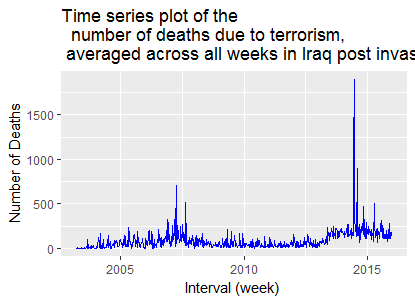
\includegraphics[width=10cm]{Peters_experiment_markdown_files/figure-latex/Rplot03_weekly_death_counts_iraq.png}
\caption{Time series plot interval(week) of deaths}
\label{fig:tseriesweek}
\centering
\end{figure}

Initial Application of the Twitter outbreak algorithm was applied to terrorist deaths in Iraq, over death count data in the GTD pertaining to Iraq, from the Post invasion period upto the pullout and post-pullout . Using the twitter breakout detection algorithm, the algorithm was applied using a minimum number of transitions between change points of four weeks (approximately month). This seemed to be a reasonable time period (other periods were also trialled but appeared to influnece the results little) so as to survey counts and compare to a minimum of four weeks previously. The time series plot over-layed with the detected outbreaks is shown in figure~\ref{fig:tseriesweektwitter outbreak} 

\begin{figure}[t]
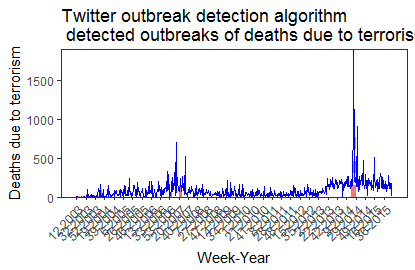
\includegraphics[width=10cm]{Peters_experiment_markdown_files/figure-latex/Rplot02_Twitter_outbreak_detection_algo.png}
\caption{Time series plot interval(week) of deaths and application of twitter outbreak detection algorithm. The detected outbreaks are shown indicated as vertical red lines}
\label{fig:tseriesweektwitter outbreak}
\centering
\end{figure}

The breakout detection algorithm showed a number of  breakout of incidents upto the surge, break outs are seen approximately 6 months after the invasion, these breakouts become frequent after this initial period with a break out occurring more frequently upto the surge and after and post-pullout at the time of the major ISIS offensive. It should be noted that no outbreak is detected post surge till the last week in 2012. A table of identified breakouts in Iraq is shown in table~\ref{tab:labelsiraq}. 

Outbreaks are detected almost immediately after the invasion, however they seem to be extremely intermittent. Outbreaks are again detected at the end of 2003 and at the start of 2004. Outbreaks again are seen at the start 2007, which would correlate with the surge. An outbreak again is detected midway through 2007 which would correlate with the period of the US troop surge in Iraq. It is interesting to note that no outbreak (corresponding to mean or gradual shift downward trend in violence) is detected in the period post surge (late 2007 to 2008). 

The same dataset was examined using the SURUS RAD algorithm. The detected outliers are shown in Figure~\ref{fig:tseriessurusrad}. The low rank signal is represented in blue and is a pretty decent approximation of the underlying trend bar the outliers, which are represented as red circles with the size representing the magnitude of the outlier. The green line represents the underlying noise in the signal. The table detailing the outliers are in table~\ref{tab:RADTABLE}. The magnitude of the outlier is denoted in the S\_ Transform column. A high frequency of outliers are detected throughout 2006, this is correlated with the heightening of a bitter sectarian war in Iraq and the coming to the fore of AL-Qa'ida in Iraq as the pre-eminent Sunni armed opposition to the US led invasion \citep{fearon2007iraq}. The US troop surge \citep{ricks2009gamble} is also correlated with a large number of outliers in deaths due to terrorism. There is also a high frequency of outliers at the start of 2013. What is particularly interesting is that the number of  outliers increases in 2013 to 2014 and decreases in 2015.  While there is no outliers detected from mid 2007 to 2009 and mid 2009 to 2014, which would indicate their was no extremes in activity over this period.


\begin{figure}[t]
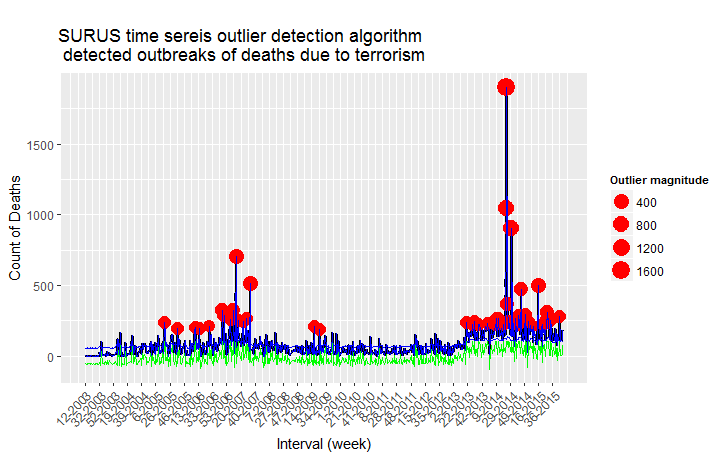
\includegraphics[width=10cm]{Peters_experiment_markdown_files/figure-latex/Surus_Rad_iraq.png}
\caption{Time series plot interval(week) of deaths and application of SURUS RAD algorithm.}
\label{fig:tseriessurusrad}
\centering
\end{figure}


\subsection{The use of syndromic surveillance methods (EARSC3 and Farrington surveillance methods) to analyse Iraqi Death counts due to terrorism} 

As stated previously both EARSC3 and Farrington's syndromic surveillance algorithm were applied to the Iraq data. In both cases, the only data preparation required was minimal, with the dataframe of counts (of deaths due to terrorism) by week requiring casting as an sts (surveillance time series) object before applying the surveillance algorithm. The output though as with the previous plots (of the SURUS outlier detection algorithm and the twitter outbreak detection algorithm) were enhanced by plotting them with ggplot, as the plotting functionality provided by the base package lacked clarity and the resulting plots were difficult to understand. For the EARSC3 algorithm, a baseline of 18 weeks (4 months roughly) was chosen (which roughly responds to a  quadrimestral review period, this was also used for the Farrington algorithm). The detected syndromic surveillance outbreaks using the EARSC3 method are shown in figure~\ref{fig:tseriesEARSC3RAD}. A table showing the alarms raised by algorithm EARSC3 are shown in \ref{tab:tseriesEARSC3RADtable}. The plot shows the alarms raised (indicating an outbreak) as red circles, the count of deaths is shown as the black line and the blue line represents the threshold. Similar to the behaviour noted with the outlier detection algorithm, post the US troop surge in 2007 there is a relatively small amount of outbreaks detected till 2009, only one in 2010 and after that a steady increase in outbreaks till 2014 and into 2015 when the number of detected outbreaks begins to decrease.

\begin{figure}[t]
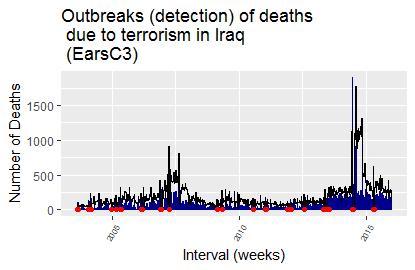
\includegraphics[width=10cm]{Peters_experiment_markdown_files/figure-latex/Rplot02_EarsC3.png}
\caption{Time series plot interval(week) of deaths and application of EARSC3 algorithm}
\label{fig:tseriesEARSC3RAD}
\centering
\end{figure}

The output of the Farrington algorithm is shown in figure~\ref{fig:tseriesFarrington} and the table of outbreaks is shown in table~\ref{tab:tseriesEARSC3RADtable}. The output of the Farrington algorithm is quite similar to that of the EARSC3 algorithm except the algorithm fails to observe the outbreak that was noted at the end of April/ start of May 2013 and also no outbreaks are observed to occur in 2015. The Farrington algorithm detects far less outbreaks than are detected using the EARSC3 methodology, while both use the same review period. The Farrington algorithm was implemented using a B parameter of 0 so as to  include only 0 years back in time, i.e the current window so as to allow a direct comparison with the EARSC3 method which only uses data specified in the current window, allowing a like with like comparison of detected outbreaks. This would suggest that the Poisson regression over estimated the baseline values (from which the outbreaks are ascertained) or else the C statistic used in the EARSC3 method is not sensitive enough to noise and is being exceeded too often because of this. This would be due to the methodology not taking account of specific characteristics of count data such as over dispersion \citep{sellers2013data}, which is accounted for by the Farrington model.

Also as the methodology is an unsupervised learning problem (the detection of aberrations in time series data), multiple methods are often used together and if multiple algorithms are tripped their is stronger evidence for an outbreak \citep{reis2003time}. An alarm plot, figure~\ref{fig:alarmplot1} shows the performance of both algorithms, showing alarms raised by both the EarsC and Farrington method. Figure~\ref{fig:alarmplot2} shows the output of all models (EarsC, Farrington, SURUS and RAD) overlayed on top of each other this allows the deconstruction of the time series by the comparing of the alarms raised by the different methods. For instance if and alarm is raised which detects a syndromic outbreak coincides with an alarm raised by RAD, this can be further classified as an outbreak due to an outlier. While, if an alarm is raised which detects a syndromic outbreak coincides with an alarm raised by SURUS, this can be further classified as an outbreak due mean or gradual shifts. It's also interesting to note that during the post surge period (late 2007-2008) while a number of (syndromic) outbreaks are detected no outliers or EDM detected outbreaks are detected (see figure~\ref{fig:CaptureAlarmPlot3}).

Comparison to real world events (such as major insurgent offensives) and/or by an expert in the field (of terrorism or counter terrorism) could also be used to judge the effectiveness of the methods in detecting outbreaks of terrorism. 


\begin{figure}[t]
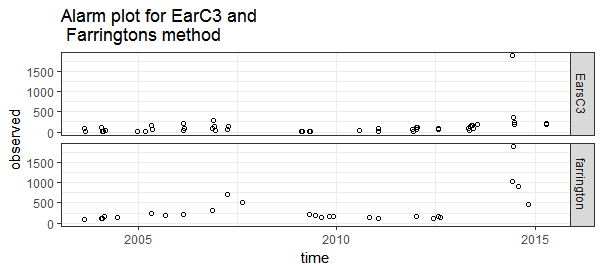
\includegraphics[width=10cm]{Peters_experiment_markdown_files/figure-latex/Rplot03alarmplotfarringtonearsC3.png}
\label{fig:alarmplot1}
\centering
\caption{Alarm plot for Farringtons and EarsC3 syndromic surveillance methods.}
\end{figure}


\begin{figure}[t]
\includegraphics[width=10cm]{Peters_experiment_markdown_files/figure-latex/Rplot03alarmplotfarringtonearsC3_SURUS_RAD.png}
\label{fig:alarmplot2}
\centering
\caption{Alarm plot for Farringtons, EarsC3, SURUS and RAD method syndromic and aberration detection methods.}
\end{figure}


\begin{figure}[t]
\includegraphics[width=10cm]{Peters_experiment_markdown_files/figure-latex/CaptureAlarmPlot3.png}
\label{fig:CaptureAlarmPlot3}
\centering
\caption{Alarm plot for Farringtons, EarsC3, SURUS and RAD method syndromic and aberration detection methods, overlayed with the time series plot.}
\end{figure}


\begin{figure}[t]
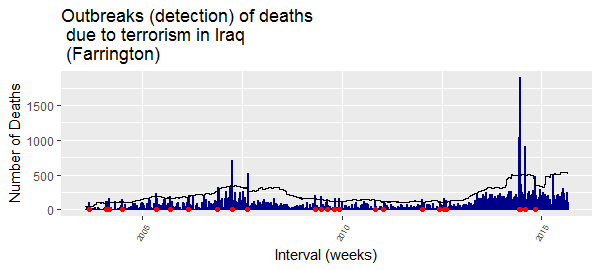
\includegraphics[width=10cm]{Peters_experiment_markdown_files/figure-latex/Rplot02_Farrington_detected_Outbreaks.png}
\label{fig:tseriesFarrington}
\centering
\caption{Time series plot interval(week) of deaths and application of Farrington algorithm}
\end{figure}

\section{Surveying multiple countries or regions at the same time using purrr}

Using the different methodologies on the Iraq dataset it was possible to detect \textit{'interesting time events'} whether they were outbreaks or time series outliers. As previously stated (see section~\ref{sec:chap5intro}), the benefit of using these methodologies is there generalizability, as they do not have to be supplemented with additional data or (as is the case with HMM's) require extensive analysis to make sense of. Instead the outbreak and anomaly detection algorithms used in this chapter highlight where \textit{'interesting time events'} occur. The models also have the benefit in that they can be further generalized by using functional programming to apply them to individual countries or regions. Using this approach, it is possible to carry out a mass survey of regions, locations and highlight outbreaks of terrorism in these areas. This is achieved through the use of purrr package \citep{purrrWickham2016} in R. 

The purrr package \citep{wickham2016r} increases R's functional programming capabilities by implementing a set of capabilities for working with functions, vectors. Of particular use is the map function which allows instead of looping over a vector, carrying out an operation and saving the results. This minimizes the amount of code that needs to be written and allows the code to be generalized further. In the analysis code map() is used to split a dataframe by country and fit a outlier detection model to each subset of data and extract the output of where the outbreak events occurred. This is achieved through code similar to that shown in listing~\ref{fig:purrrlabel}: 

\begin{figure}
\begin{verbatim}
subset_models <- sbsetmideast %>%
  split(
    .$country_txt
  ) %>%
  map(~ breakout(.$sum_kill, min.size=12, 
            method='multi', percent=.1, 
            degree=1, plot=FALSE)) %>%
    map("loc")  
\end{verbatim}
\caption{Applying the SURUS model functionally by mapping it across different countries and extracting the dataframe locations of the outbreak.}
\label(fig:purrrlabel)
\end{figure}

Explaining listing~\ref{fig:purrrlabel} the sbsetmideast dataframe is segmented by country (the time series count data deaths due to terrorism is partitioned by country) using the split function. The map function is then applied to each different partition and time location (the location of the outbreaks in the time series) are outputted to a list and a dataframe of countries and the resulting list of outbreaks is outputted. This simple code listing illustrates how generalizable the methodologies are.

Once the model is applied the locations can be extracted and an alarm dataframe for all countries created using very simple functional and procedural code which could be easily placed into a simple function to make application simpler. This is achieved through code similar to that shown in listing~\ref{fig:purrrlabel2} and listing~\ref{fig:purrrlabel3}: 

\begin{figure}
\begin{verbatim}
na.pad <- function(x,len){
  x[1:len]
}

makePaddedDataFrame <- function(l,...){
  maxlen <- max(sapply(l,length))
  data.frame(lapply(l,na.pad,len=maxlen),...)
}

locs.df<-subset_models %>% map(unlist) %>% makePaddedDataFrame() 

listcountries<-unique(sbsetmideast$country_txt 

%>% as.character()) 

pl.holder.dfx<- data.frame()

for(i in listcountries){
  tsti<-sbsetmideast  %>% filter(country_txt==i)  
  country_outbreaks<-tsti[locs.df[,i],] %>% 
  filter(!is.na(year))

  tsti$outbreak<-ifelse(tsti$weekstrdate %in% country_outbreaks $weekstrdate,"outbreak","no outbreak")
  pl.holder.dfx<-rbind(pl.holder.dfx,tsti)
  }
\end{verbatim}
\caption{Processing the output of functional program to mark the dates across multiple countries the outbreak occurred.}
\label{fig:purrrlabel2}
\end{figure}

\begin{figure}
\begin{verbatim}
ggplot(pl.holder.dfx, aes(x=weekstrdate, y=sum_kill)) +
  geom_line(color = "blue")+geom_text(data=pl.holder.dfx %>% filter(outbreak=="outbreak"),aes(weekstrdate,sum_kill,label="o"))+facet_grid(country_txt ~ .)+
  ggtitle("Time series outbreak (SURUS) plot of the  \n  
  number of deaths due to terrorism, \n 
  averaged across all weeks in 
  Iraq, Syria, Yemen, Jordan post Iraq invasion")+
  xlab("Interval (week) ")+
  ylab("Number of Deaths")
\end{verbatim}
\caption{Plotting the output of the SURUS accross multiple countries using ggplot.}
\label{fig:purrrlabel3}
\end{figure}


This code simply unlists the dates of the outbreaks by country and creates a dataframe based off these. Then using a for loop, creates a column with a marker if an outbreak is detected. Finally the results are plotted using ggplot faceted by country. This faceted plot is shown in figure~\ref{fig:tseriesSURUSmulcountry}. 

\begin{figure}[t]
\includegraphics[width=10cm]{Peters_experiment_markdown_files/figure-latex/Rplot03_multiple_countries_SURUS_RAD.png}
\label{fig:tseriesSURUSmulcountry}
\centering
\caption{Time series plot interval(week) of deaths and application of SURUS algorithm across multiple countries in the mid-east}
\end{figure}

\section{Discussion}
Preliminary modelling of count of deaths due to terrorism either using count regression techniques or count time series modelling techniques proved problematic. Regression models suffered from incorrect specification. For the count regression models the models suffered from over dispersion.  Also the data held within the GTD was not sufficient on its own and had to be integrated with additional data regarding presidential reigns of US and Iraqi presidents along with coalition troop deployment and withdrawls.  HMM’s were also experimented with for modelling count (deaths due to terrorism) time series data. 

HMM’s proved very useful in defining periods or epochs of high terrorism or low terrorism, however they suffered from lack of generalizability as the number of transition states would have to be empirically derived per country or region (or the preferences of an analyst) being analysed.  

To overcome this problem a number of different methods were used which are used to model ‘interesting’ count time series events. Typical events of this type include:
\begin{itemize}
\item Mean shifts. These are step changes are characterized by sudden shifts, which result in large continuous change when compared to previous time series events.
\item Gradual shifts or ramp ups which are steady and slow changes between two levels.
\item Outliers, these are data points which are far from other observations in the dataset.
\item Outbreaks, these are the sustained occurrences (of an indefinite time period) of terrorist events (in this case deaths due to terrorism) over what would normally be expected in a specific region, country or community.
\end{itemize}

Statistical methods are used to uncover all of the above defined terms.  To uncover, mean shifts or gradual shifts the twitter outbreak detection algorithm (SURUS) is used. SURUS uses E divisive with  means (EDM), which is a methodology which makes use of energy statistics to detect large departures from the median. A benefit of using this methodology is that it makes no underlying assumptions about the underlying distributions as it makes use of robust statistics. 

To elucidate the presence of outliers,  Netflix’s RAD \citep{pylypenkocognitive} algorithm is used to detect time series outliers.  RAD works in two components, firstly it creates an array of features composing of the time series lag correlation, seasonality and spectral entropy, from this PCA is then performed to detect outliers (these are points that are for removed from the highest density regions). Another benefit of using this type of methodology is that similarly to the EDM method, it is non-parametric.

Lastly syndromic surveillance methods which are primarily used to detect disease outbreaks are applied to the study of outbreaks in terrorism. An outbreak in this sense is the manifestation of terrorist events or deaths which exceed what would be normally expected. An outbreak can last for an indefinite period and for that reason is particularly addressing the research question of interest in this thesis, the detection of changes in intensity associated with terrorism particularly an increase in intensity of terrorism (due to deaths or incidents). As changes in behaviour are ill defined one would not want them to be restricted to certain time series events but be able to detect sustained changes or short lived changes, this makes surveillance methods specifically suited to detecting outbreaks in terrorists deaths. Both Farrington’s and the EarsC3 methods were used to monitor outbreaks of terrorism. Both methods function by establishing a baseline and if this is exceeded an outbreak is detected. The C3 method is particularly useful when working with data that does not have alot of historic values as only data is required from the recent past to function \citep{stacey2007comparison}. 

Both methods differ in their approach to outbreak detection. Farrington’s method for every time point in the series predicts the number of deaths due to terrorism using a GLM, which is then compared to the actual count of deaths and if this observation exceeds an analyst specified quantile of the prediction interval an alarm is triggered by the algorithm. The EarsC3 method works differently by comparing each point to a threshold calculated from time points in a period in the immediate past (the length of this period is determined by the analyst). 

The threshold is then compared to the observed value and as with the Farrington method, if the observed value is greater than an arbitrary (again determined by the analyst) quantile of the prediction interval, an alarm is triggered.  

The application of these surveillance methods requires little tuning (with the exception of setting specific alpha levels), are easy to understand and can be generalized easily. Also as a syndromic outbreak is defined not as a mean shift, gradual shift or an outlier but as an observation outside that of above an expected baseline value under normal conditions it is better suited to answering the specific research question is it possible to detect a change in intensity of terrorism (a rather non-specific term), in terms of increases of incidents or deaths due to terrorism. 

However when used in conjunction with EDM and time series outbreak detection it allows further classification of outbreaks if detected. A further benefit of using these methods is that they are not only highly generalizable when used with specific functional programming paradigms within R they can be applied across many different regions. This makes them particularly useful for the task of surveying many different countries or regions at once for changes in intensity of terrorism in an automated (due to the methods being highly generalizable) fashion.  After the outbreaks are detected they can either be assessed by a subject matter expert or additional analysis carried out and combined with the surveillance analysis to give a better understanding of the nature of the outbreaks. 

By combining with other count time series anomaly detection methods outbreaks can be further classified as mean shifts, gradual shifts or outbreaks. For example EarsC3 algorithm detected an Outbreak from 2014-06-09 to 2014-06-30, during the same period at weeks 25,27,31 and 34 of 2014 the RAD algorithm detected outbreaks occurring, while the SURUS \citep{kelly2015propagating} outbreak detection methods detected a mean shift occurring during week 22 and 26 of 2014. Almost immediately after the surge (late 2007 - 2008) outbreaks are detected using the syndromic surveillance methods and time series anomalies are detected following the US troop surge in 2007.

It should be noted that compared to the syndromic surveillance methods the EDM based methods fail to detect a number of outbreaks detected by the syndromic surveillance methods. This may be due to the use of robust statistical methods by the SURUS algorithm which do not posses the necessary sensitivity to detect outbreaks detected by the syndromic surveillance methods. 

While the methods were easy to generalize and apply across multiple countries or regions, there are weaknesses to their implementation particularly in R, that is the visualization methods associated with them are implemented in Base R graphics and are sparse and not very clear to implement. While the data could be visualized in ggplot, it must be done so by writing custom visualization code and not using a native visualization function within the surveillance package (it would be extremely useful if the authors of this package rewrote the visualization functions using ggplot). 

The second problem associated with the use of the surveillance methods is the count time series data must be cast as a sts (surveillance time series object) which consists of subsets of slots within in it containing observed, population and state \citep{hohle2007r}. The sts object is quite complex in structure and it’s hierarchical nature can be difficult to interact with for analysts more used to working with flatter data structures more common in data analysis such as data frames, data tables, or time series objects (such as R’s ts or xts data structure).

\section{Conclusion}

A number of methods for exploring the detection of \textit{'interesting count time series events'} for the purpose of detecting changes in behaviour (particularly intensity) of terrorism were explored. 4 methodologies were tested, that tested for particular time series aberration events; outbreaks, outliers, gradual and mean shifts.  

These methods proved easier to both apply and interpret than the methods originally explored in the preliminary analysis. Also unlike the previous methods they did not suffer from problems associated with incorrect specification (in the case of the regression models). The methods were also more easy to generalize with little if any parameters having to be tuned and using functional programming paradigms which exist in R, specifically the purrr package, their application to multiple countries or even administrative regions is relatively easy.

The methods used in this chapter are also complimentary to each other, as when a an outbreak is detected using the syndromic surveillance methods they can be further classified using the other methods as either outliers or mean shifts or gradual shifts.
